
\documentclass[12pt]{article}
\usepackage{times}
\usepackage{setspace}
\setstretch{1.5}
\usepackage{amsmath,amssymb, amsthm}
\usepackage{graphicx}
\usepackage{bm}
\usepackage[hang, flushmargin]{footmisc}
\usepackage[colorlinks=true]{hyperref}
\usepackage[nameinlink]{cleveref}
\usepackage{footnotebackref}
\usepackage{url}
\usepackage{listings}
\usepackage[most]{tcolorbox}
\usepackage{inconsolata}
\usepackage[papersize={8.5in,11in}, margin=1in]{geometry}
\usepackage{float}
\usepackage{caption}
\usepackage{esint}
\usepackage{url}
\usepackage{enumitem}
\usepackage{subfig}
\usepackage{wasysym}
\newcommand{\ilcode}{\texttt}
\usepackage{etoolbox}
\usepackage{physics}
\usepackage{xcolor}
\patchcmd{\thebibliography}{\section*{\refname}}{}{}{}



\makeatletter
\renewcommand{\@seccntformat}[1]{}
\makeatother

\begin{document}



\title{\textbf{CSDS 440: Assignment 5}}

\author{Shaochen (Henry) ZHONG, \ilcode{sxz517} \\ Mingyang TIE, \ilcode{mxt497}}
\date{Due on 10/09/2020, submitted \textcolor{blue}{early} on 10/02/2020 \\ Fall 2020, Dr. Ray}
\maketitle


% % % % % % % % % % % % % % % % % % % % % % % % % % % % % % % % % %
% % % % % % % % % % % % % % % % % % % % % % % % % % % % % % % % % %
% % % % % % % % % % % % % % % % % % % % % % % % % % % % % % % % % %
\section{Problem 19}

\begin{align*}
    b^T u &= u^T b \\
    &\leq u^T \cdot Ax \ \ \text{(Since $Ax \geq b$)}\\
    c^T X &= x^T c \\
    &\geq x^T A^T u \ \ \text{(Since $A^u \leq c$)}\\
    &\geq u^T Ax \\
    \Longrightarrow \ b^T u &\leq c^T X
\end{align*}

The statement is therefore proven.

% % % % % % % % % % % % % % % % % % % % % % % % % % % % % % % % % %
% % % % % % % % % % % % % % % % % % % % % % % % % % % % % % % % % %
% % % % % % % % % % % % % % % % % % % % % % % % % % % % % % % % % %
\section{Problem 20}



% % % % % % % % % % % % % % % % % % % % % % % % % % % % % % % % % %
% % % % % % % % % % % % % % % % % % % % % % % % % % % % % % % % % %
% % % % % % % % % % % % % % % % % % % % % % % % % % % % % % % % % %
\section{Problem 21}

Note for the following neural network, the weights are noted on the edges and the activation thresholds are noted on the top of each neuron (as for the neuron with threshold $x$ will output $+1$ if the input $\geq x$, and output $-1$ otherwise). Note we omitted $x_2$ as it is simply a duplication of $x_1$, and we can design a network without using the former.

\begin{figure}[H]
    \centering
    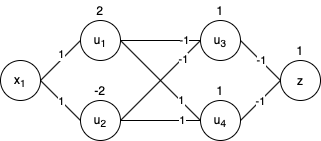
\includegraphics[width=0.4\linewidth]{{fig/fig_p21.png}}
\end{figure}

Now to trace each example. Note for each neuron, the inequality is the input against the activation threshold and the one in bracket represents the output.
\begin{table}[H]
\centering
    \begin{tabular}{|rr|rrrr|r|}
        \hline
        $x_1$ & $x_2$ & $u_1$ & $u_2$ & $u_3$ & $u_4$ & $z$ \\
        \hline
        -4 & -4 & $-4<2$ (-1) & $-4< -2$ \ (-1) & $1 + 1 > 1$ \ (1) & $-1 - 1 < 1$ \ (-1) & $-1 + 1 < 1$ \ (-1) \\
        -1 & -1 & $-1<2$ \ (-1) &$-1> -2$ \ (1)  & $1 - 1 < 1$ \ (-1) & $1 - 1 < 1$ \ (-1) & $1 + 1 > 1$ \ (1) \\
        1 & 1 &  $1<2$ \ (-1) &  $1>-2$ \ (1)& $1 - 1 < 1$ \ (-1) & $1 - 1 < 1$ \ (-1) & $1 + 1 > 1$ \ (1) \\
        4 & 4 & $4>2$ (1) & $4>-2$ \ (1) & $1 - 1 < 1$ \ (-1) & $1 + 1 > 1$ \ (1) & $1 - 1 < 1$ \ (-1) \\
        \hline
    \end{tabular}
\end{table}

We have showed the network is able to produce the correct classification.


% % % % % % % % % % % % % % % % % % % % % % % % % % % % % % % % % %
% % % % % % % % % % % % % % % % % % % % % % % % % % % % % % % % % %
% % % % % % % % % % % % % % % % % % % % % % % % % % % % % % % % % %
\section{Problem 22}




% % % % % % % % % % % % % % % % % % % % % % % % % % % % % % % % % %
% % % % % % % % % % % % % % % % % % % % % % % % % % % % % % % % % %
% % % % % % % % % % % % % % % % % % % % % % % % % % % % % % % % % %
% \section{References}
% \nocite{*}
% \raggedright
% \bibliography{references.bib}
% \bibliographystyle{plain}


\end{document}